\begin{minipage}[c]{.6\linewidth}
La société Sharp commercialise des caisses automatiques utilisées par exemple dans des boulangeries. Le client glisse directement les billets ou les pièces dans la machine qui se charge de rendre automatiquement la monnaie. 
\begin{obj}
Afin de satisfaire les clients, on cherche à déterminer un algorithme qui va permettre de rendre le moins de monnaie possible. 
\end{obj}
\end{minipage}\hfill
\begin{minipage}[c]{.37\linewidth}
\begin{center}
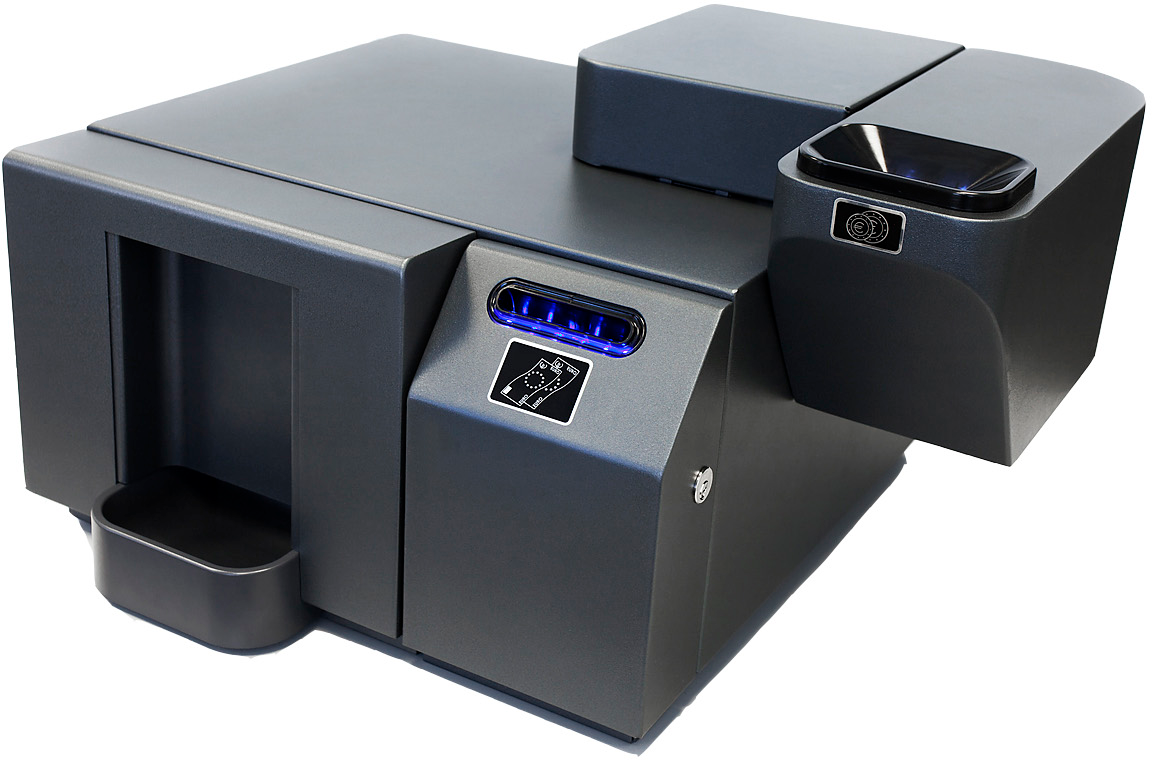
\includegraphics[width=.9\textwidth]{sharp.png}
\end{center}
\end{minipage}

%\setcounter{subparagraph}{0}

La machine dispose de billets de 20€, 10€ et 5€ ainsi que des pièces de 2€, 1€, 50, 20, 10, 5, 2 et 1 centimes. 

On se propose donc de concevoir un algorithme qui demande à l'utilisateur du programme la somme totale à payer ainsi que le montant donné par l'acheteur. L'algorithme doit alors afficher quels sont les billets et les pièces à rendre par le vendeur. 

%\question{}Créer une liste {valeurs} contenant toutes les valeurs des billets ou pièces.

%\question{}
%Pour un montant d'achat donné et pour une somme donnée par le client, proposer un algorithme en pseudo code permettant de rendre le minimum de monnaie au client. Cet algorithme devra détailler la somme à rendre (nombre de pièces et nombre de billets).

\question{}
Justifier le fait d'utiliser une structure de liste pour gérer les valeurs des billets ou des pièces. La mettre en place et la nommer \pyv{valeurs}.


\question{}
Ecrire une fonction \pyv{rendre_monnaie(cout,somme_client,valeurs)} prenant en arguments deux flottants \pyv{cout} et \pyv{somme_client} représentant le coût d'un produit et la somme donnée par le client en € ainsi que \pyv{valeurs}. Cette fonction renverra une liste \pyv{nombre_billets} qui donnera pour chaque terme de \pyv{valeurs} le nombre de pièces et/ou billets à rendre.

\question{} Créer une fonction \pyv{afficher_rendu_monnaie(cout,somme_client,valeurs)} permettant d'afficher le nombre de pièces et billets à rendre comme l'exemple ci-dessous.

\begin{center}
\begin{lstlisting}
afficher_rendu_monnaie(15.99,17.5,valeurs)

0 : billet de 20 euros
0 : billet de 10 euros
0 : billet de 5 euros
0 : pièce de 2 euros
1 : pièce de 1 euros
1 : pièce de 50 centimes
0 : pièce de 20 centimes
0 : pièce de 10 centimes
0 : pièce de 5 centimes
0 : pièce de 2 centimes
1 : pièce de 1 centimes
\end{lstlisting}
\end{center}



%\question{}
%Quel type de variable est il préférable d'utiliser pour décompter l'argent ? Pourquoi ?
%
%\question{}
%Implémenter cet algorithme dans Python.
%
%\question{}
%Vérifier sur plusieurs cas que l'algorithme fonctionne.